\documentclass{report}
\usepackage{fancyhdr} % Required for custom headers
\usepackage{lastpage} % Required to determine the last page for the footer
\usepackage{extramarks} % Required for headers and footers
\usepackage{graphicx} % Required to insert images
%\usepackage{lipsum} % Used for inserting dummy 'Lorem ipsum' text into the template
\usepackage{amsmath}
\usepackage{float}
\usepackage{graphicx} 
%\usepackage{amsfont}
%\usepackage{amssymb}

\usepackage{multicol}
% Margins
\topmargin=-0.5in
\evensidemargin=0in
\oddsidemargin=-0.5in
\textwidth=7.5in
\textheight=9.0in
\headsep=0.25in 


\pagestyle{fancy}

%\rhead{\textbf{Marshall's Recipes}} % Top right header
%\lhead{\textbf{Curry Stir Fry}}
%\chead{ }
%\title{Curry Stir Fry}

\begin{document}
%\vspace{8mm}
%\textbf{PRELIMINARIES:}


\bigskip

\bigskip

\begin{multicols}{2}
\textbf{Ingredients}
\begin{itemize}
\item 1 onion \quad (45 kCal/ 1 gP/ 0 gF/ 11 gC)
\item 2 lbs stew beef \newline(2274 kCal/ 234 gP/  138 gF/ 0 gC)
\item 1 can diced tomatoes \quad (93 kCal/ 2 gP/ 0 gF/ 23 gC)
\item 2 medium zucchini \quad (66 kCal / 6 gP / 2 gF / 12 gC)
\item 3 russet potatoes (medium/medium large) \quad (504 kCal/ 15 gP/ 0 gF/ 111 gC)
\item 1 lb baby carrots \quad (186 kCal / 4 gP / 0 gF / 45 gC)
\item 2 cans tomato sauce (8 oz each) \quad (106 kCal / 8 gP / 0 gF / 22 gC)
\item 1 can of corn (with water) \quad (280 kCal/ 7 gP/ 5 gF/ 32 gC)
\item $\sim 5$ cloves of garlic (minced) (65 kCal / 3 gP/ 0 gF/ 15 gC) 
\item 4-5 cups of water (enough to fill $\frac{1}{4}$ inch from rim of crock pot.)

\item 6-7 cubes of beef bullion 
\item 2 tsp. salt (more to taste) 
\item 1 tsp. black pepper
\item 1 tsp. thyme
\item 3 bay leaves 


\end{itemize}


\columnbreak
\textbf{Procedure:}
\medskip


\begin{enumerate}
\item \textbf{\textit{Note:}}This is a MASSIVE recipe. This will fill an 8-quart slow cooker to the brim. 
\item Dice onion, cube potatoes and beef, chop carrots in half, cut zucchini into bite-sized pieces. Add to crock pot. Add canned items, bullion, and spices then fill with water and give it a good stir. 


\medskip
\item Cook on low in crock pot for approximately 8 hours for best results. I usually start it in the morning to have it ready for dinner. 
  
\end{enumerate}
\begin{table}[H]
  \begin{center}
    \caption{Macro totals}
    \label{tab:table1}
    \begin{tabular}{c|c|c|c} % <-- Alignments: 1st column left, 2nd middle and 3rd right, with vertical lines in between
      \textbf{Calories} & \textbf{Protein} & \textbf{Fat} & \textbf{Carbs}\\
      \hline
      3,510 kCal & 280 g & 145 g & 271 g\\
    \end{tabular}
  \end{center}
\end{table}
\end{multicols}




%\begin{center}
%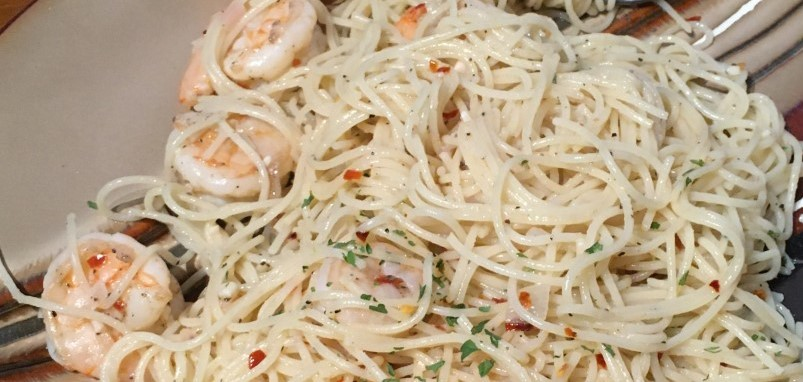
\includegraphics[scale=0.65]{Pasta/Shrimp Scampi/Shrimp Scampi.jpg}
%\end{center}


\end{document}